%%%%%%%%%%%%%%%%%%%%%%%%%%%%%%%%%%%%%%%%%%%%%%%%%%%%%%%%%%%%%%%%%%%%%%%%%%%%%%%%%%
\begin{frame}[fragile]\frametitle{}
\begin{center}
{\Large Notes from Teachings of Krishna Prakash of Shrimath}
\end{center}
\end{frame}

%%%%%%%%%%%%%%%%%%%%%%%%%%%%%%%%%%%%%%%%%%%%%%%%%%%%%%%%%%%
\begin{frame}[fragile]\frametitle{Starting Yoga}

	\begin{itemize}
	\item Yoga Sadhna is An Endless Ocean	
	\item You cannot be a Yoga Teacher/Guru just after training or certification, practice it for years (12), experience the benefits, then only teach.
	\item Small Sized Yoga Classes is a Must
	\item Meditation instructions lack emphasis on posture.
	\item Still Your Body and Steady Mind
	\item Persist with spiritual practices Long Enough
	\item Guru emphasizes endless hours, and dedication for yoga.
	\item Without steadiness, meditation cannot happen e.g. curd sets when still
	\item Asana brings steadiness and Pranayama brings lightness, pratyahara brings witness-bhava
	\item Pavanmuktasana series by Satyananda, of 34 Asanas To Start Yoga Journey
	\end{itemize}

{\tiny (Ref:  I Did yoga for 7 Days Following A Yogi's Advice- With ‪@ShrimathYoga‬  spirituality - Tathastu - Secrets of Bharat)}

\end{frame}

%%%%%%%%%%%%%%%%%%%%%%%%%%%%%%%%%%%%%%%%%%%%%%%%%%%%%%%%%%%
\begin{frame}[fragile]\frametitle{Immunity}

\begin{columns}
    \begin{column}[T]{0.6\linewidth}
		\begin{itemize}
		\item 340 important pressure points on the body with which health can be managed. 28 are on palms. Clapping for upto 20 minutes before meals
		\item 'PraN Mudra' (thumb and last two small fingers touching) 12 minutes
		\item 'Ling Mudra' (fist clasped, left thumb upward, keep at naval) 12 minutes
		\item Bhramari Pranayam + Khechari Mudra, inhale without sound, exhale with bee sound from tight throat. 7 minutes, 3 times a day.
		\end{itemize}

    \end{column}
    \begin{column}[T]{0.4\linewidth}
		\begin{center}
		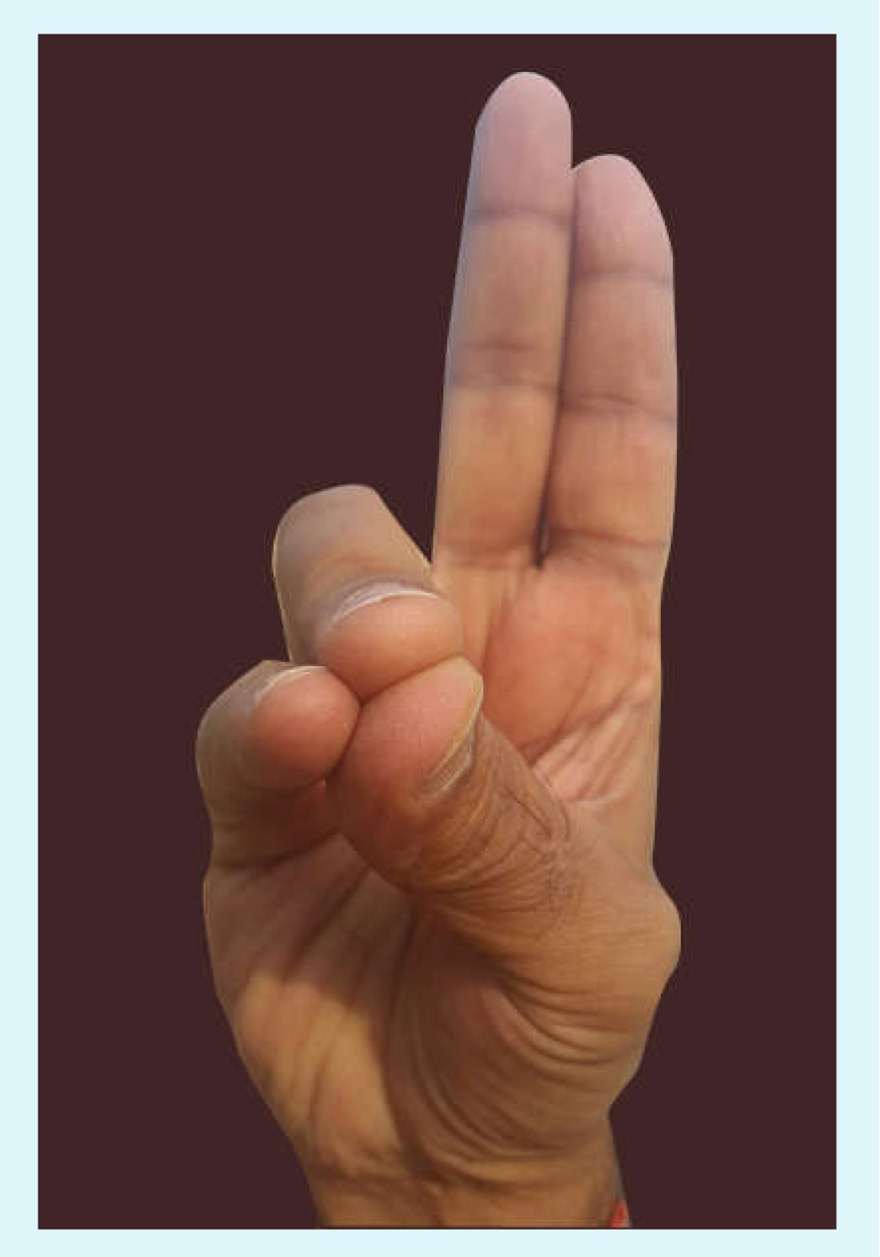
\includegraphics[width=0.4\linewidth,keepaspectratio]{pranmudra}
		
		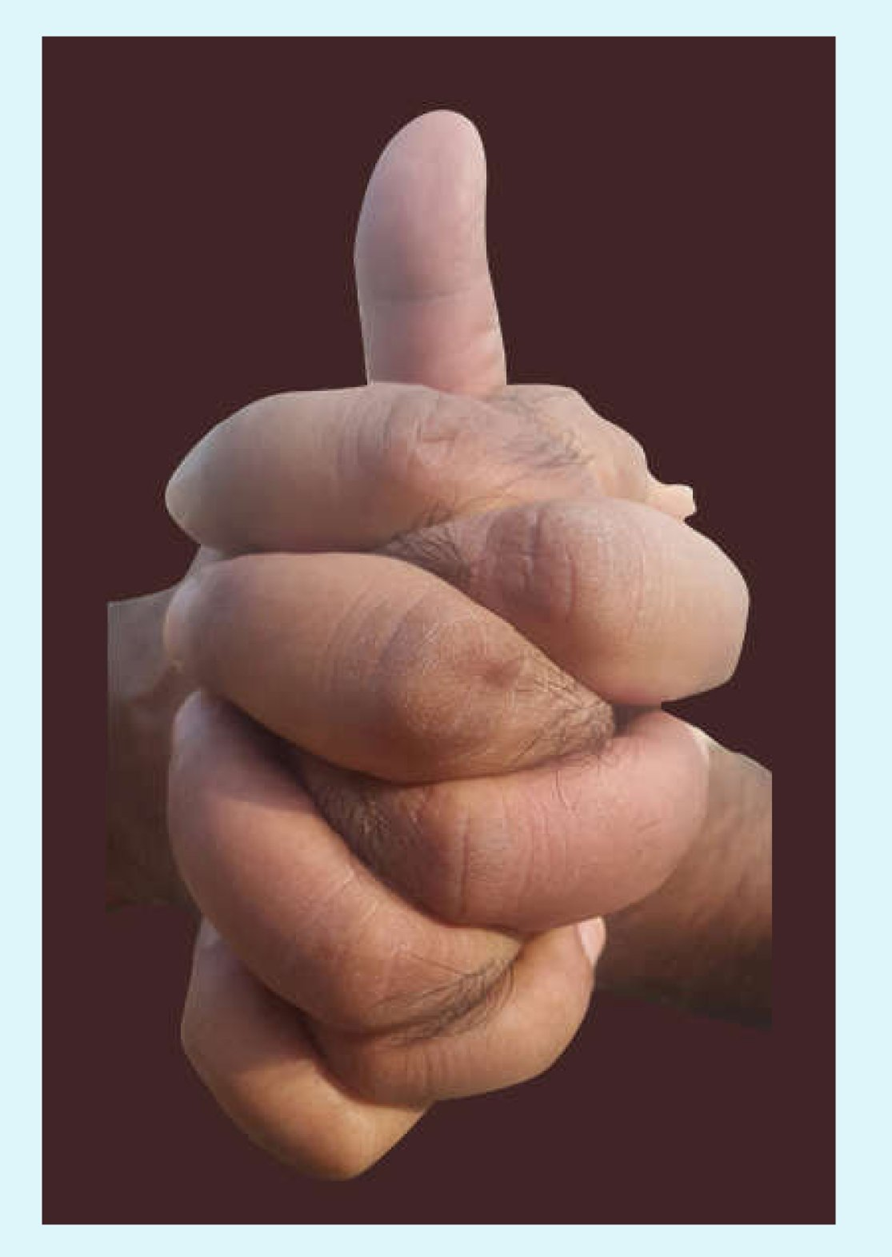
\includegraphics[width=0.4\linewidth,keepaspectratio]{lingmudra}
		
		\end{center}	
    \end{column}
  \end{columns}
  


{\tiny (Ref:  Building Immunity 2.0 - Shrimath Yoga)}

\end{frame}

%%%%%%%%%%%%%%%%%%%%%%%%%%%%%%%%%%%%%%%%%%%%%%%%%%%%%%%%%%%
\begin{frame}[fragile]\frametitle{Inner Silence}


		\begin{itemize}
		\item Part of Pratyahara (withdrawal of senses).
		\item Our attributes: We always seek to know, we wish to live forever and know what we dont know, even gossip is ok. We want to be happy.
		\item Level 1: learn to live with sensory pulls and pushes. Accept distractions. Going to retreat is running away from reality. We cannot change 'outside'. Be immune to it by being aware. Stand there in the problems. Be witness like a traffic police.
		\item Summary:
			\begin{itemize}
			\item Lesser thoughts
			\item Clarity in thought without confusion.
			\item Lack of prejudice and being open.
			\item Ability to stay calm even when triggered 
			\item Non judgmental and not jumping to conclusions even without listening and knowing about a subject.
			\end{itemize}
		\end{itemize}

{\tiny (Ref:  Master Class on Antar Mouna Level 1 - Shrimath Yoga)}

\end{frame}


%%%%%%%%%%%%%%%%%%%%%%%%%%%%%%%%%%%%%%%%%%%%%%%%%%%%%%%%%%%%%%%%%%%%%%%%%%%%%%%%%%
\begin{frame}[fragile]\frametitle{}
\begin{center}
{\Large Tapping Grace through Yoga Nidra}
\end{center}
\end{frame}

%%%%%%%%%%%%%%%%%%%%%%%%%%%%%%%%%%%%%%%%%%%%%%%%%%%%%%%%%%%
\begin{frame}[fragile]\frametitle{Part 1}

\begin{itemize}
    \item Take every situation as a boon from the divine. For example, Covid brought people together and gave a new perspective on life.
    \item Divinity works in five ways:
    \begin{itemize}
        \item Creation (Brahma)
        \item Sustenance-Maintenance (Vishnu)
        \item Dissolution-Destruction (Shiva) to enable new creation
        \item Veiling (Tirodhana): The illusion that external things bring happiness (e.g., "If I have money, I will be happy"). This illusion drives action, reaction, and over-action.
        \item Grace (Kripa, Anugraha): When one sincerely asks within ("Who am I?") to know the truth, grace is experienced. Just as one needs to tune into a specific station to hear a song—though the waves are always present—there are many processes to tap into grace, one of which is Yoga Nidra.
    \end{itemize}
\end{itemize}

\end{frame}

%%%%%%%%%%%%%%%%%%%%%%%%%%%%%%%%%%%%%%%%%%%%%%%%%%%%%%%%%%%
\begin{frame}[fragile]\frametitle{Part 2}

\begin{itemize}
    \item U-N-I-V-E-R-S-E: "You and I"—just one of the worlds. By grace, you can tap into abundance.
    \item Operate from a state of fullness (Purnataa).
\end{itemize}

\end{frame}

%%%%%%%%%%%%%%%%%%%%%%%%%%%%%%%%%%%%%%%%%%%%%%%%%%%%%%%%%%%
\begin{frame}[fragile]\frametitle{Part 3}

\begin{itemize}
    \item You can give only if you have it, or you must ask a bank to give.
    \item The cosmos is a bank of infinite wealth and grace.
    \item We must make ourselves eligible for this grace.
\end{itemize}

\end{frame}

%%%%%%%%%%%%%%%%%%%%%%%%%%%%%%%%%%%%%%%%%%%%%%%%%%%%%%%%%%%
\begin{frame}[fragile]\frametitle{Part 4}

\begin{itemize}
    \item We can receive only if the source has it, i.e., Purnataa.
    \item Something appearing blank does not mean it is empty. Even space has the capacity to be full.
\end{itemize}

\end{frame}

%%%%%%%%%%%%%%%%%%%%%%%%%%%%%%%%%%%%%%%%%%%%%%%%%%%%%%%%%%%
\begin{frame}[fragile]\frametitle{Part 5}

\begin{itemize}
    \item To tap into grace, you need awareness.
    \item Just BE—wherever you are, however you are, whatever you are—and observe with a non-judgmental attitude what is happening around you.
    \item For example, a traffic police officer or a judge observes in a detached manner, without being judgmental.
    \item Awareness is similar to mindfulness, heartfulness, and living in the present moment.
\end{itemize}

\end{frame}

%%%%%%%%%%%%%%%%%%%%%%%%%%%%%%%%%%%%%%%%%%%%%%%%%%%%%%%%%%%
\begin{frame}[fragile]\frametitle{Part 6}

\begin{itemize}
    \item Accepting fullness is better than trying to empty the mind.
    \item The mind is vast—the subconscious is immense. It is not possible to empty all its contents.
    \item Reality is infinite. Thoughts cannot be counted.
    \item Just be the witness.
    \item Whether empty or full does not matter, as long as you live in the present moment.
\end{itemize}

\end{frame}

%%%%%%%%%%%%%%%%%%%%%%%%%%%%%%%%%%%%%%%%%%%%%%%%%%%%%%%%%%%
\begin{frame}[fragile]\frametitle{Part 7}

\begin{itemize}
    \item Indian traditions provide not just theory but also practical processes.
    \item Yoga Nidra is the practice of developing a witness attitude and a state of acceptance.
    \item It helps manage stress and desires while promoting relaxation.
\end{itemize}

\end{frame}

%%%%%%%%%%%%%%%%%%%%%%%%%%%%%%%%%%%%%%%%%%%%%%%%%%%%%%%%%%%
\begin{frame}[fragile]\frametitle{Part 8}

\begin{itemize}
    \item Yoga Nidra helps manifest desires.
    \item We walk through life with a veil (curtain) and thus do not see reality.
    \item By fulfilling desires through Yoga Nidra, we begin to believe in the practice. Continued practice deepens the attitude of witnessing.
    \item We realize that process orientation is more important than results. Many factors determine outcomes, and much is beyond our direct control.
\end{itemize}

\end{frame}

%%%%%%%%%%%%%%%%%%%%%%%%%%%%%%%%%%%%%%%%%%%%%%%%%%%%%%%%%%%
\begin{frame}[fragile]\frametitle{Part 9}

\begin{itemize}
    \item Once we become aware, we start living in the present moment.
    \item Anxiety is neutralized.
    \item We realize that we must do our best and accept whatever happens.
    \item A contented mind subdues its fluctuations and perturbations.
    \item A calm and contented mind becomes eligible to receive grace (the fifth mode).
\end{itemize}

\end{frame}

%%%%%%%%%%%%%%%%%%%%%%%%%%%%%%%%%%%%%%%%%%%%%%%%%%%%%%%%%%%
\begin{frame}[fragile]\frametitle{Part 10}

\begin{itemize}
    \item We all need to know how to tap into grace, regardless of our differences.
    \item Seeking knowledge and truth is common to all.
    \item Peace and prosperity manifest when grace falls upon us.
\end{itemize}

\end{frame}

%%%%%%%%%%%%%%%%%%%%%%%%%%%%%%%%%%%%%%%%%%%%%%%%%%%%%%%%%%%
\begin{frame}[fragile]\frametitle{Part 11}

\begin{itemize}
    \item Yoga Nidra is a skill developed progressively.
    \item It builds mental capacity and stamina to remain still, alert, and aware.
    \item Preparatory levels provide calmness, relaxation at both physical and mental levels, steady breath flow, and a quiet mind.
\end{itemize}

\end{frame}

%%%%%%%%%%%%%%%%%%%%%%%%%%%%%%%%%%%%%%%%%%%%%%%%%%%%%%%%%%%
\begin{frame}[fragile]\frametitle{Part 12}

\begin{itemize}
    \item Yoga Nidra was introduced by Swami Satyananda to complement the practices of Yogasana and Pranayama.
    \item Passed on to Niranjanananda, it has now spread worldwide.
\end{itemize}

\end{frame}

%%%%%%%%%%%%%%%%%%%%%%%%%%%%%%%%%%%%%%%%%%%%%%%%%%%%%%%%%%%
\begin{frame}[fragile]\frametitle{Part 13}

Yoga Nidra Instructions (\ldots)

\end{frame}

%%%%%%%%%%%%%%%%%%%%%%%%%%%%%%%%%%%%%%%%%%%%%%%%%%%%%%%%%%%
\begin{frame}[fragile]\frametitle{Part 14}

\begin{itemize}
    \item Yoga Nidra restores remote control of our emotions to us.
    \item Awareness and witnessing help filter which emotions we allow to impact us.
    \item Yoga Nidra helps fulfill deep desires that define us and our lives.
    \item The next step is to move into the state of 'Just Be.'
\end{itemize}

\end{frame}



